\documentclass[aps,prd,reprint,floatfix,nofootinbib]{revtex4-2}
\usepackage{amsmath,amssymb,bm,booktabs,graphicx,microtype}
\usepackage[hidelinks]{hyperref}

\begin{document}

\title{Topology Is Not a Particle Label: A Typed-State Requirement for a Filament Particle Taxonomy}
\author{Meridian Calder}
\affiliation{SAT/H(s)H Sandbox Geometry Program}
\date{27 September 2026}

\begin{abstract}
A historical SAT Particle Zoo source assigns particle flavor to resonance mode,
places multiple flavors in common filament classes, represents force carriers
as ripples or transitions, and represents baryons as braided composites.
These definitions imply a simple but consequential formal restriction:
particle identity cannot be represented faithfully by carrier topology alone.
We state a minimal typed-state decomposition and demonstrate the
non-injectivity geometrically with an explicit harmonic filament family whose
carrier topology is unchanged while curvature, torsion, and arclength vary.
A separate exact three-strand representative demonstrates that the stated
braid geometry can be generated reproducibly while also exposing the need for
endpoint, framing, and binding conventions before assigning a particle-specific
topological invariant.  The result is a source-faithful taxonomy constraint,
not a claim that the historical particle identifications are physically realized.
\end{abstract}

\maketitle

\section{Source-derived typing problem}

The controlling historical source for this note is
\texttt{SATv THE PARTICLE ZOO.txt}.
It describes fermions as persistent filaments, particle flavor as a resonance
mode, quarks as short high-curvature filament segments that bind into braided
composites, leptons as longer singly curved filaments, neutrinos as near-aligned
filaments, and bosons as ripples or structural transitions.

These are not all the same mathematical object type.  A minimal state is
therefore
\begin{equation}
X=(C,F,G,E,B,P),
\end{equation}
where $C$ is carrier class, $F$ is framing/topological data, $G$ is metric or
differential geometry, $E$ is excitation/phase state, $B$ is binding/composite
relation, and $P$ is persistence/event type.

Let $\pi_C:X\rightarrow C$ retain only the carrier class.
Because the source distinguishes flavors through resonance/excitation or
geometry while retaining the same broad carrier class,
the particle-labeling map is not injectively recoverable from $\pi_C$ alone.

\section{Calculated same-topology family}

Consider the family of embedded filament segments
\begin{equation}
\gamma_n(s)=
\left(
R\cos ns,\,
R\sin ns,\,
ps
\right),
\qquad
0\le s\le 4\pi ,
\label{eq:helix}
\end{equation}
for positive integers $n$.
Every member has interval carrier topology, while
\begin{align}
\kappa_n&=\frac{Rn^2}{R^2n^2+p^2},\\
\tau_n&=\frac{pn}{R^2n^2+p^2}.
\end{align}
Thus geometry and harmonic state can vary while carrier topology is unchanged.

\begin{figure}[t]
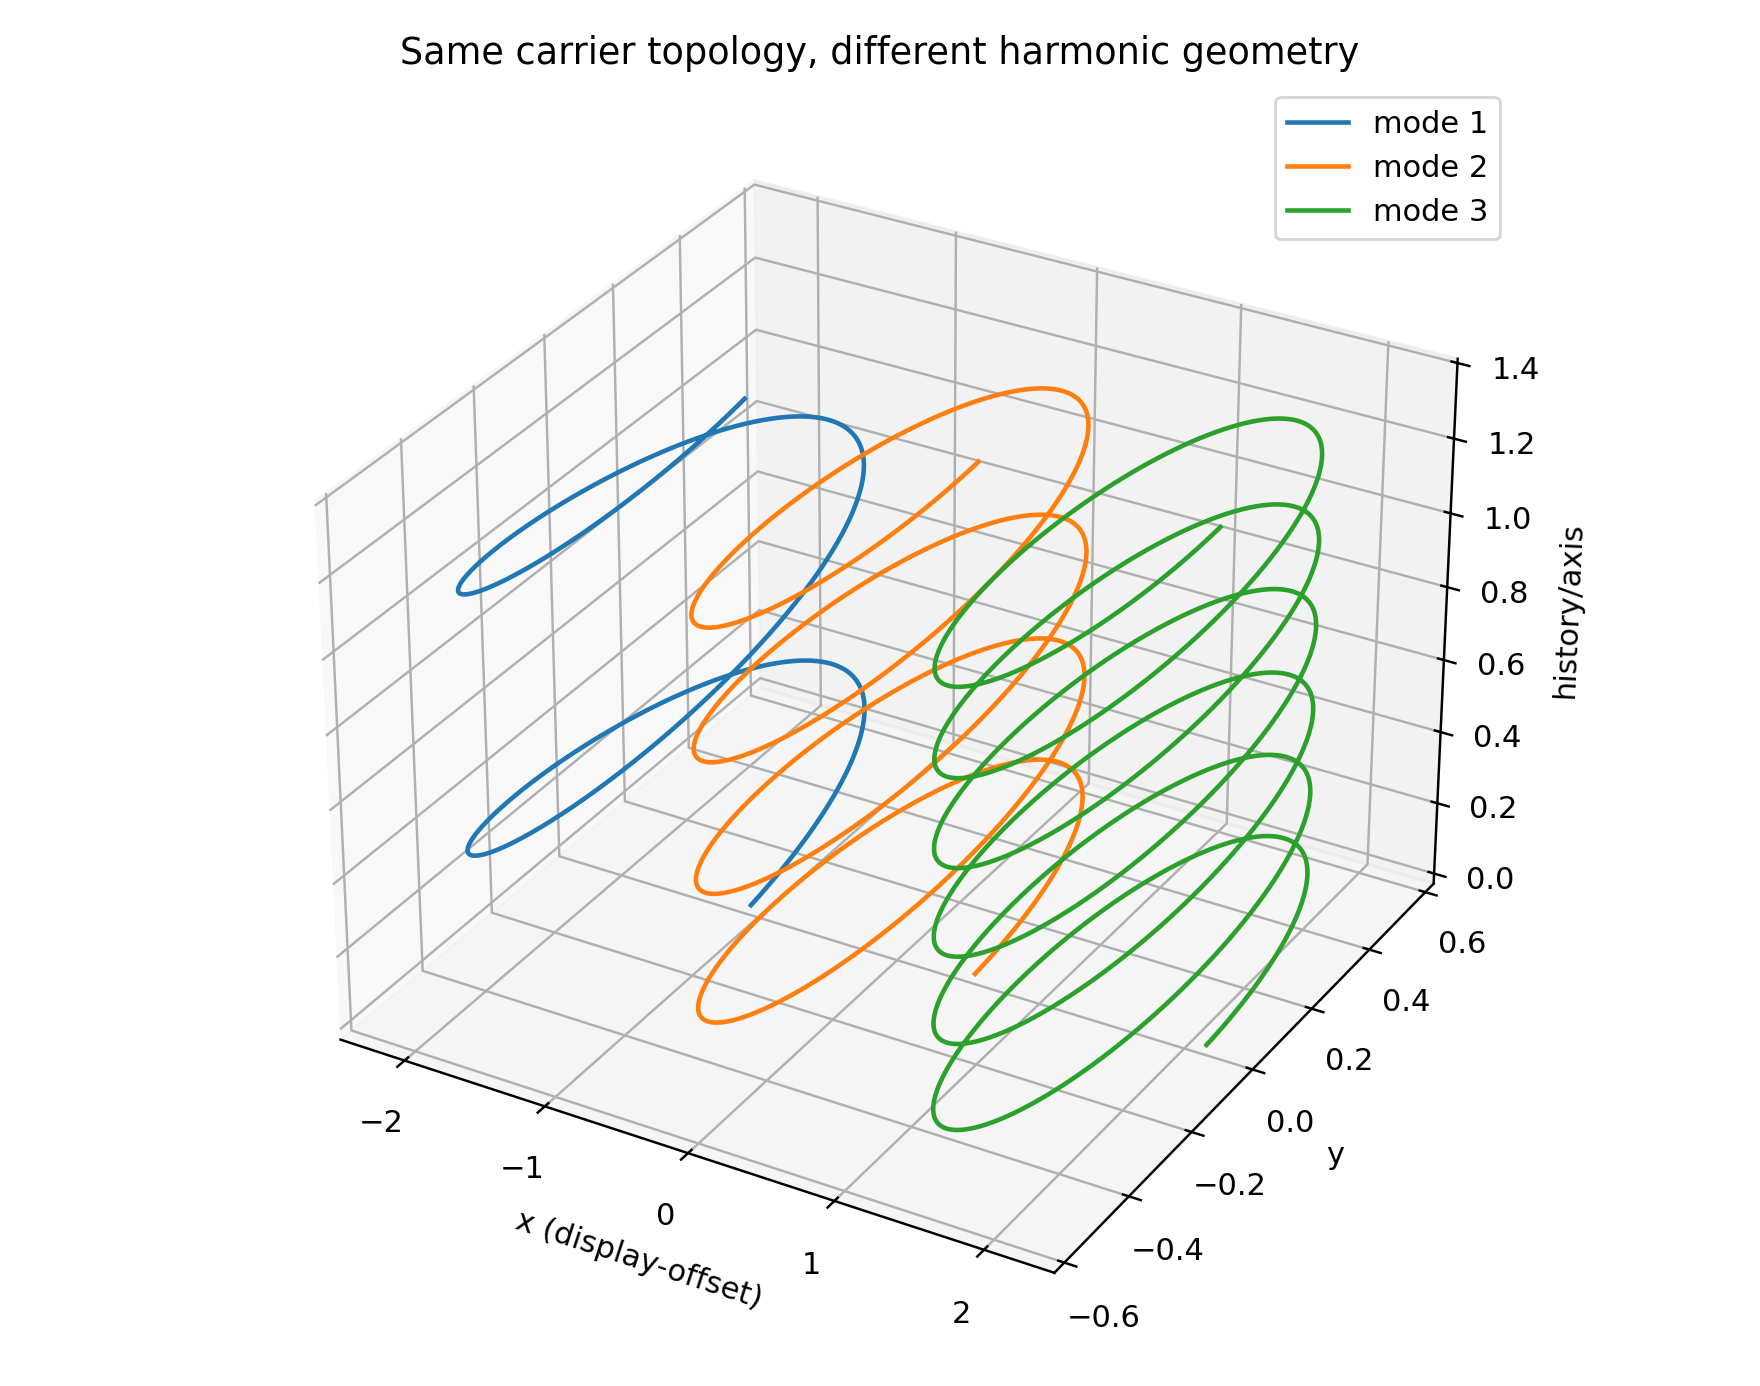
\includegraphics[width=\columnwidth]{zoo_same_topology_different_geometry.png}
\caption{Three exact members of Eq.~(\ref{eq:helix}), displayed with lateral
offsets only for legibility.  The construction is a representative realization
of the historical source's ``harmonic'' distinction, not a fitted
electron--muon--tau model.}
\end{figure}

\section{Braided composite representative}

The source describes a baryonic composite as three braided quark filaments.
A minimal exact representative is
\begin{equation}
\begin{aligned}
\bm\beta_j(z)
&=\bigl(
R_b\cos(2\pi z+2\pi j/3),\\
&\qquad
R_b\sin(2\pi z+2\pi j/3),\,z
\bigr),\\
&\hspace{2.5em}j=0,1,2,
\end{aligned}
\label{eq:braid}
\end{equation}
for $0\le z\le1$.
At equal $z$, every strand pair is separated by
\begin{equation}
d=\sqrt{3}\,R_b,
\end{equation}
which supplies a direct numerical regression check.

For open strands, the topology depends on what is held fixed at the boundary
and on whether framing is part of the state.  A centerline alone also does not
record ribbon or worldtube twist.  Particle-specific topological assignments
therefore require endpoint, framing, binding, and readout conventions beyond
the carrier curves in Eq.~(\ref{eq:braid}).

\begin{figure}[t]
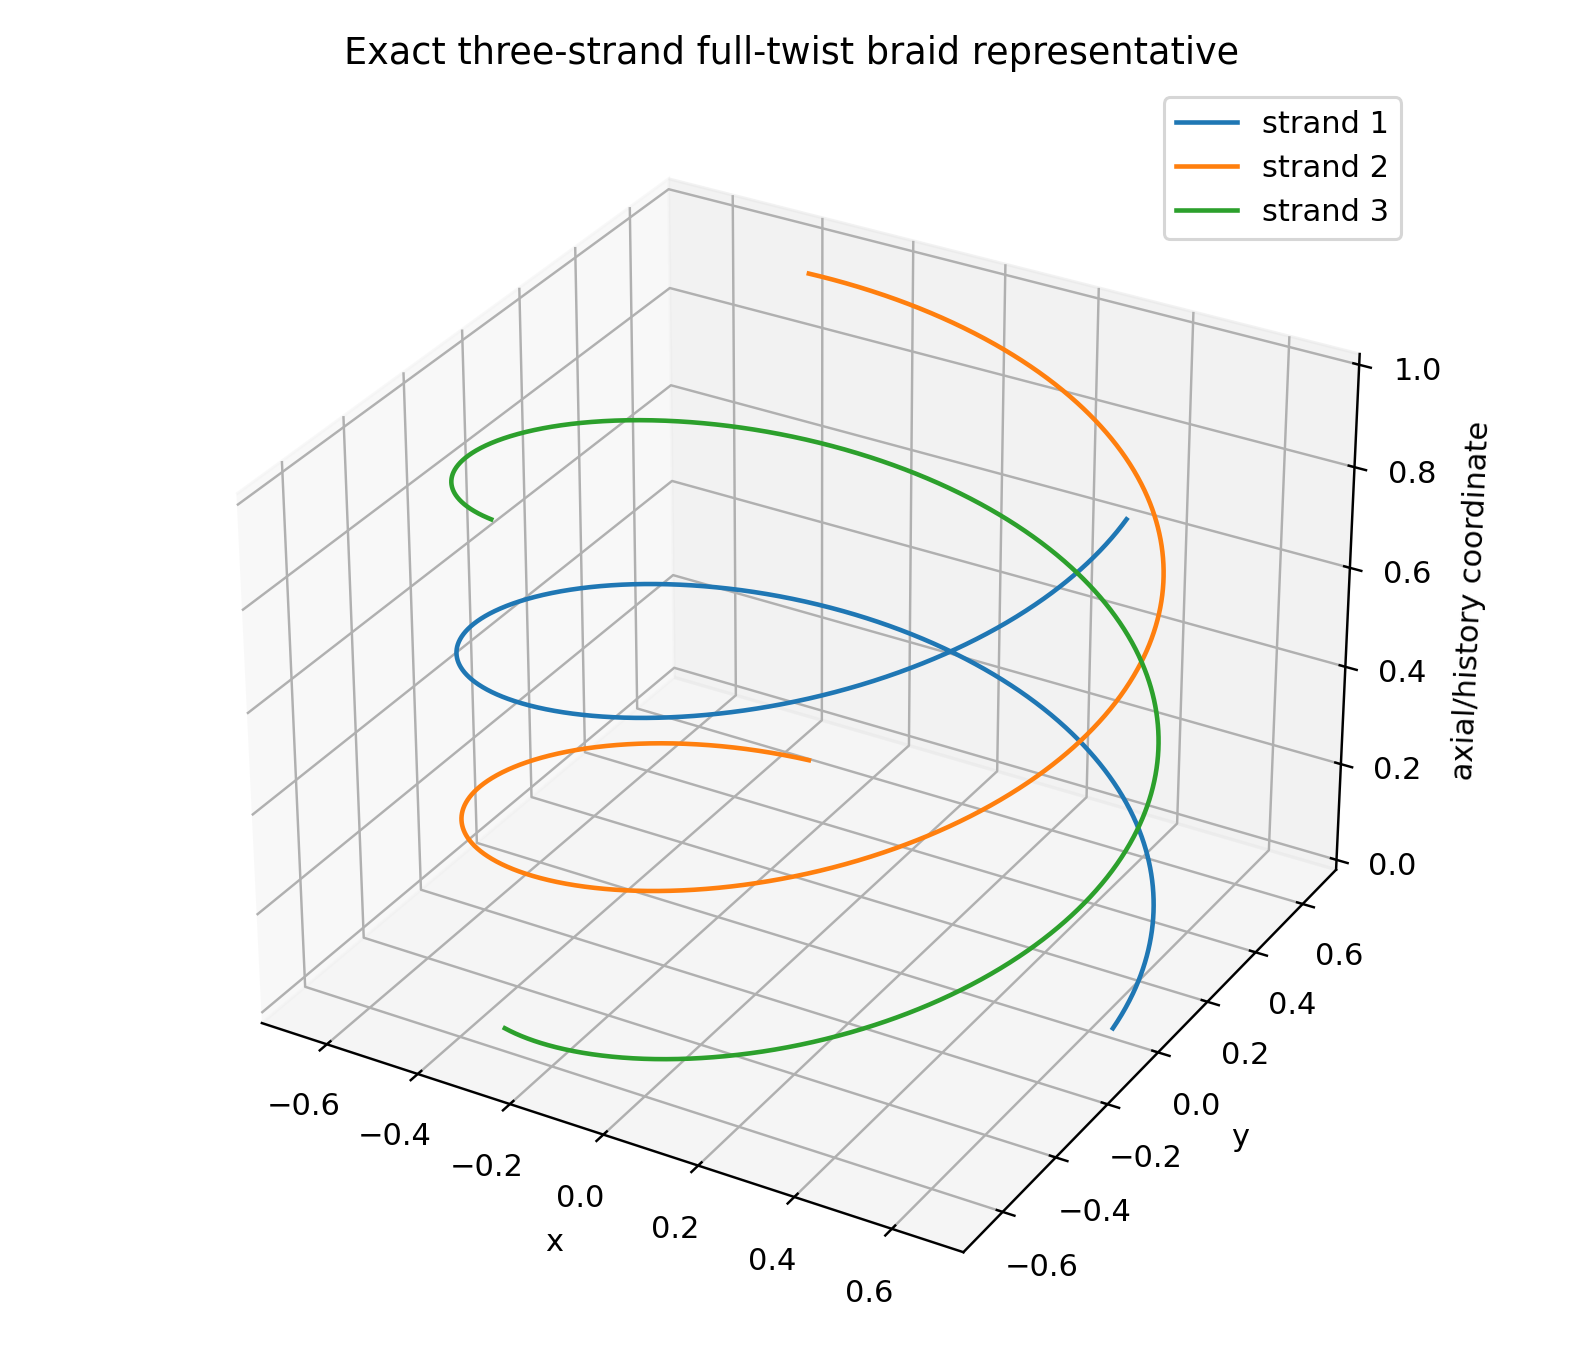
\includegraphics[width=\columnwidth]{zoo_three_strand_braid.png}
\caption{Exact three-strand full-twist representative from Eq.~(\ref{eq:braid}).
It realizes the stated three-filament braid geometry but is not, by itself,
a proton or neutron identification.}
\end{figure}

\section{Related use cases}

Topological particle taxonomies using braids or knots have precedents, including
Bilson-Thompson, Hackett and Kauffman's braided-belt construction,
Finkelstein's quantum-knot program, and Asselmeyer-Maluga's braid/3-manifold
constructions.  These are comparison points for mathematical use-case only;
no equivalence to SAT/H(s)H is asserted.

\section{Consequence for solver design}

A Particle Zoo solver should return a typed state rather than a single topology
label.  In particular, the implementation should not force a unique knot or
braid invariant onto a particle whose source definition distinguishes it by
resonance, curvature, phase, or composite binding.  This separation permits
topological invariants to be used where defined while retaining metric and
dynamical information required by the source taxonomy.

\begin{thebibliography}{9}

\bibitem{BTHK2009}
S.~O. Bilson-Thompson, J. Hackett, and L.~H. Kauffman,
``Particle Topology, Braids, and Braided Belts,''
\textit{J. Math. Phys.} \textbf{50} (2009),
doi:10.1063/1.3237148.

\bibitem{Finkelstein2007}
R.~J. Finkelstein,
``The Elementary Particles as Quantum Knots in Electroweak Theory,''
\textit{Int. J. Mod. Phys. A} \textbf{22} (2007),
doi:10.1142/S0217751X0703707X.

\bibitem{Asselmeyer2019}
T. Asselmeyer-Maluga,
``Braids, 3-Manifolds, Elementary Particles,''
\textit{Symmetry} \textbf{11} (2019),
doi:10.3390/sym11101298.

\end{thebibliography}

\end{document}
